\documentclass[eng,oneside]{mgr}
\usepackage[polish]{babel}
\usepackage[utf8]{inputenc}
\usepackage{polski}
\usepackage[hidelinks]{hyperref}
\usepackage{graphicx} 
\usepackage{listings}
\usepackage{color}
\frenchspacing
\usepackage{indentfirst}
\usepackage{caption}

\definecolor{mygreen}{rgb}{0,0.6,0}
\definecolor{mygray}{rgb}{0.5,0.5,0.5}
\definecolor{mymauve}{rgb}{0.58,0,0.82}

\lstset{
	backgroundcolor=\color{white},   % choose the background color
	basicstyle=\footnotesize,        % size of fonts used for the code
	breaklines=true,                 % automatic line breaking only at whitespace
	frame=single,  
	commentstyle=\color{mygreen},    % comment style
	escapeinside={\%*}{*)},          % if you want to add LaTeX within your code
	keywordstyle=\color{blue},       % keyword style
	stringstyle=\color{mymauve},     % string literal style
}

\author{Marcin Mantke}
\title{System zarządzania inteligentnym domem z wykorzystaniem Raspberry Pi oraz technologii internetowych.}
\engtitle{Smart house management system using Raspberry Pi and Web technologies.}
\supervisor{dr inż. Marek Piasecki}
\field{Informatyka (INF)}
\specialisation{Inżynieria systemów informatycznych (INS)}
\date{2015}

\begin{document}
\maketitle
\tableofcontents
\chapter{Wstęp}
\section{Ogólny opis pracy}
Inteligentny dom, który monitoruje warunki panujące w środku, może samodzielnie sterować wieloma urządzeniami i elementami budynku, zna nasze zwyczaje i z którym możemy nawet porozmawiać, dla wielu jest zagadnieniem rodem z filmów sc-fi. Ale czy rzeczywiście tak jest? 

Od kilkunastu lat możemy zaobserwować znaczny rozwój wszystkich dziedzin techniki, a przez to technologii, które są wykorzystywane w inteligentnych budynkach. Wiele urządzeń, z których korzystamy na co dzień i które pracują niezależnie od innych urządzeń (dobrym przykładem jest ekspres do kawy), posiadają interfejsy, dzięki którym możemy podłączyć je do internetu i zdalnie nimi zarządzać. Korzystając z przykładu wcześniej wymienionego ekspresu do kawy, wracamy z pracy, wiemy o której godzinie będziemy w domu i możemy zdalnie ,,zlecić mu'' zaparzenie kawy, aby od razu po powrocie na nas czekała. A gdyby nasz dom rzeczywiście znał nasze zwyczaje? Odpowiedź jest prosta - kawa czekałaby na nas dokładnie wtedy, kiedy byśmy mieli na nią ochotę.

Inteligentne budynki, to nie tylko wygoda. To również spore oszczędności finansowe. Zwykle temperatura jest regulowana jedynie na podstawie temperatury panującej obecnie w budynku/danym pomieszczeniu. Co gdyby wziąć pod uwagę inne parametry? System inteligentnego domu zwykle zbiera dużo więcej parametrów niż tylko temperatura. Poprzez analizę tych parametrów możemy tak sterować ogrzewaniem, ale również innymi parametrami budynku, że w skali roku zaoszczędzimy na tym niekiedy niemałe pieniądze.

Jak widać, rozwiązania z zakresu inteligentnych budynków niosą za sobą wręcz nieograniczone możliwości. Obecnie, w czasach gdzie elementy elektroniczne są szeroko dostępne, wiedza z zakresu elektroniki, automatyki i informatyki jest coraz bardziej powszechna, a największym ograniczeniem jest ludzka wyobraźnia, inteligentne domy mają świetny czas, aby stać się czymś tak powszechnym. Tak powszechnym, jak zwykłe komputery, które jeszcze kilkanaście lat temu były czymś wyjątkowym i dla wielu osób zbędnym. A dzisiaj nie potrafią bez nich żyć.
\section{Cel pracy}
% Celem projektu jest zaprojektowanie, zamodelowanie, implementacja i wdrożenie systemu zarządzania inteligentnym domem działającym w oparciu o technologie internetowe i Raspberry Pi.
Realizację projektu można podzielić na cztery etapy:
\begin{enumerate}
	\item projektowanie,
	\item modelowanie,
	\item implementację i testowanie,
	\item wdrożenie systemu.
\end{enumerate}
Powyższe etapy składają się na pełny proces powstawania systemu informatycznego. Głównym celem projektu jest realizacja każdego z tych etapów, co wymaga zapoznania się ze standardami oraz technologią i ich praktycznym wykorzystaniem. Cel ten jest osiągnięty poprzez stworzenie systemu zarządzania inteligentnym domem. System ten łączy 3 obszary techniki: informatykę, elektronikę oraz automatykę. Jego interdyscyplinarność wymaga przynajmniej podstawowej wiedzy z każdego z obszarów.

Metytorycznym celem pracy jest zapoznanie się z nowoczesnymi i bardzo przyszłosćiowymi rozwiązaniami, jakimi są inteligentne budynki. Dzięki stworzeniu platformy, która umożliwiała by niskim kosztem zmianę swojego mieszkania bądź domu w inteligentny budynek, możliwa by była znaczna popularyzacja inteligencji budynkowej. Niesie to za sobą znaczne korzyści - zarówno podniesienie komfortu życia, jak i oszczędności finansowe.

\section{Wymagania}
Głównym wymaganiem odnośnie projektu było zaprojektowanie i implementacja systemu składającego się z czujników, elementów aktywnych, jednostki centralnej, bazy danych i aplikacji webowej, w którym wszystkie elementy będą poprawnie ze sobą współpracować.

\section{Zarys koncepcji}
Koncepcyjnie, inteligentny dom można podzielić na dwie główne części. Są to czujniki i elementy aktywne oraz zintegrowany system zarządzania. Na najniższym poziomie znajdują się czujniki i elementy wykonawcze. Sensory odpowiadają za zbieranie danych na temat warunków panujących w budynku, np. temperatury i wilgotności powietrza, poziomu nasłonecznienia, stężenia dwutlenku i tlenku węgla, ruchu w pomieszczeniach. Na podstawie tych danych można sterować dużą ilością urządzeń oraz parametrów budynku. Przykładem może być sterowanie temperaturą ogrzewania i klimatyzacji, jasnością oświetlenia bądź stopniem otwarcia rolet. Kolejnym poziomem jest system zarządzania. Jest to kluczowy element systemu, który musi działać poprawnie i niezawodnie. Przyjmuje on dane z sensorów, steruje elementami aktywnymi systemu, obsługuje bazę danych i dostarcza interfejs użytkownika, ale przede wszystkim posiada algorytmy, przy pomocy których analizuje dane odebrane z czujników i odpowiednio używa elementów aktywnych.

Jak zostało wcześniej wspomniane, do tematu inteligentnych domów można podejść na dwa sposoby - hobbystycznie i komercyjnie. Biorąc pod uwagę koszt podejścia komercyjnego oraz jego względny brak elastyczności, przy realizacji projektu przyjęte zostało podejście hobbystyczne.

Jako przykład realizacji systemu zarządzania inteligentnym domem można podać system składający się z czujników, które mierzą temperaturę oraz wilgotność, symulatora elementów wykonawczych oraz systemu zarządzania. Na potrzeby pracy został zrealizowany system o takim zakresie.

\section{Przegląd wybranych rozwiązań}
\subsection{Domoticz.com}
Od czasu popularyzacji rozwiązań pokroju Arduino i Raspberry Pi, hobbystyczne projekty inteligentnych domów są coraz częściej realizowane. Sprzyja temu fakt, że ceny podzespołów wymaganych do realizacji projektu są coraz niższe, a osoby zainteresowane mają coraz więcej literatury dostępnej w Internecie. Takimi właśnie hobbystami byli twórcy platformy \textit{Domoticz}. Jest to zagraniczny serwis udostępniający multiplatformowe rozwiązania dla inteligentnych domów. Jest on skierowany głównie do hobbystów. Jak można przeczytać na stronie domowej projektu (\url{http://www.domoticz.com/}), \textit{Domoticz} jest systemem automatyki domowej, który pozwala na monitorowanie i konfigurację urządzeń, takich jak: światła, przełączniki, różnego rodzaju sensory i mierniki, jak np temperatury, deszczu, wiatru, UV, prądu, gazu i wody.

Serwis ten udostępnia biblioteki umożliwiające podłączenie sensorów oraz oprogramowanie jednostki bazowej systemu (zwykle Raspberry Pi). Jako, że udostępniane są biblioteki, a nie tylko gotowe moduły sprzętowe, całość jest bardziej elastyczna. Oczywiście są tu ograniczenia, zarówno hardware'owe, jak i software'owe, lecz są one mniejsze niż w przypadku gotowych rozwiązań.

Samo oprogramowanie jest darmowe (Licencja GNU), ze strony producenta możliwy jest zakup urządzeń współpracujących z jego systemem, jednak możliwe jest również tworzenie sensorów we własnym zakresie, przy użyciu posiadanych podzespołów oraz udostępnionych bibliotek.
\subsection{Fibaro}                                                                                              
Rozwiązania oferowane przez firmę \textit{Fibaro} mają odmienną filozofię od firmy \textit{Domoticz}. Firma ta jest ukierunkowana na rozwiązania komercyjne. Oferuje ona systemy automatyki budynkowej, składające się z gotowych podzespołów, które trzeba jedynie zainstalować w budynku oraz skonfigurować.

System umożliwia dodawanie własnych scenariuszy działania. Ich definiowanie zbudowane jest na wzór programowania \textit{Scratch} (\url{https://scratch.mit.edu/})

System Fibaro opiera się na topologii sieci typu \textit{mesh}. Urządzenia łączą się ze sobą za pośrednictwem protokołu \textit{Z-wave}.
\begin{figure}[h]
\centering
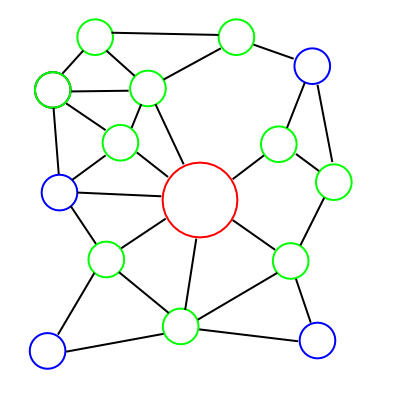
\includegraphics[width=0.4\linewidth]{mesh}
\caption{Schemat topoligii typu mesh.}
\label{fig:Mesh-Network}
\end{figure}

\chapter{Architektura systemu}
\section{Rozmieszczenie komponentów systemu}
Wszystkie komponenty systemu zostały rozmieszczone w taki sposób, aby możliwa była komunikacja pomiędzy wszystkimi elementami systemu. Aplikacja odpowiedzialna za komunikację z sensorami i elementami aktywnymi, aplikacja internetowa oraz baza danych umieszczone zostały na jednostce bazowej systemu inteligentnego domu.

Rozdzielenie wszystkich komponentów systemu naturalnie wymusiło w projekcie zastosowanie architektury 3-warstwowej:
\begin{enumerate}
	\item \textbf{warstwa prezentacji} – odpowiedzialna za prezentowanie odpowiednio przetworzonych danych użytkownikowi,
	\item \textbf{warstwa biznesowa} – na tym poziomie realizowane są wszystkie operacje biznesowe odpowiedzialne za przetwarzanie danych otrzymanych od użytkownika przed zapisaniem ich do bazy danych lub danych otrzymanych z bazy danych w celu przygotowania ich do ,,pokazania'' użytkownikowi. Są tu również przetwarzane dane przychodzące z czujników oraz wychodzące do elementów aktywnych,
	\item \textbf{warstwa dostępu do danych} – tutaj znajduje się baza danych naszej aplikacji; na tym poziomie dane przechowywane są w sposób ,,zrozumiały'' dla bazy danych.
\end{enumerate}
Rozmieszczenie komponentów systemu w danych warstwach przedstawia poniższy diagram rozmieszczenia:
\clearpage
\begin{figure}[h]
\centering
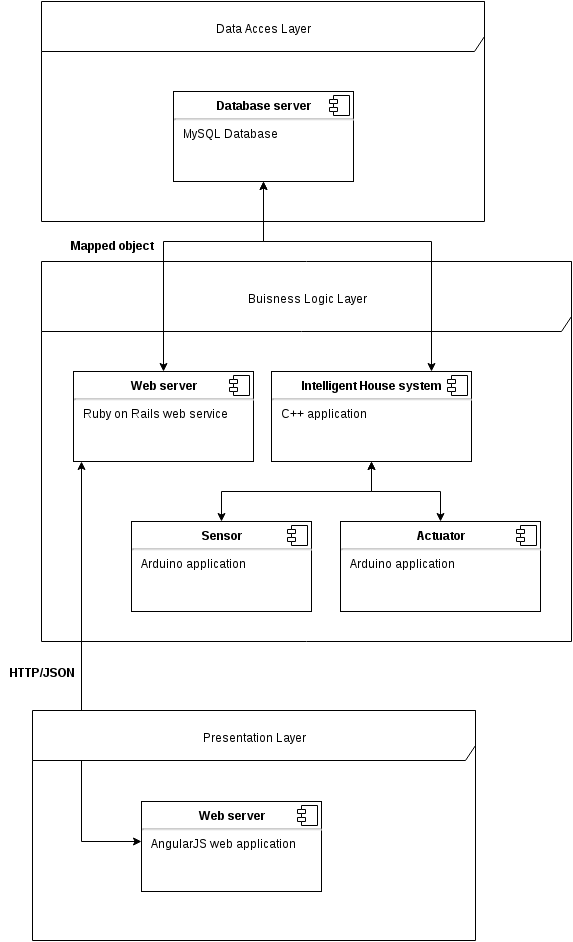
\includegraphics[width=\linewidth]{layers}
\caption{Diagram rozmieszczenia komponentów systemu.}
\label{fig:diagram_rozmieszczenia}
\end{figure}
\clearpage

\section{Topologia systemu inteligentnego domu}
Znaczna większość systemów inteligentnych domów opiera się na topologii gwiazdy. ,,Ramionami'' gwiazdy są sensory i elementy aktywne, natomiast elementem łączącym te ramiona jest system zarządzania. Zastosowanie takiej topologii ma bardzo dużą zaletę - jeśli któryś z sensorów bądź elementów aktywnych przestanie działać, to nie ma to wpływu na działanie pozostałych elementów systemu. Ponadto, dzięki zastosowaniu topologii gwiazdy, system jest bardziej wydajny. Elementy peryferyjne mają ograniczoną moc obliczeniową, a przez to ograniczoną ilość zadań, które mogą wykonać. Większa ilość zadań spoczywających na nich, wymusiłaby zwiększenie mocy obliczeniowej, co automatycznie zwiększyłoby również koszt systemu, a jest to wysoce nieporządane zjawisko. Zamiast tego część zadań należy przydzielić jednostce bazowej, która powinna być najbardziej wydajnym elementem system.


Niestety, z topologią gwiazdy wiąże się spore niebezpieczeństwo, ponieważ jeśli to jednostka bazowa ulegnie awarii, to przestaje działać cały system. 

\begin{figure}[h]
\centering
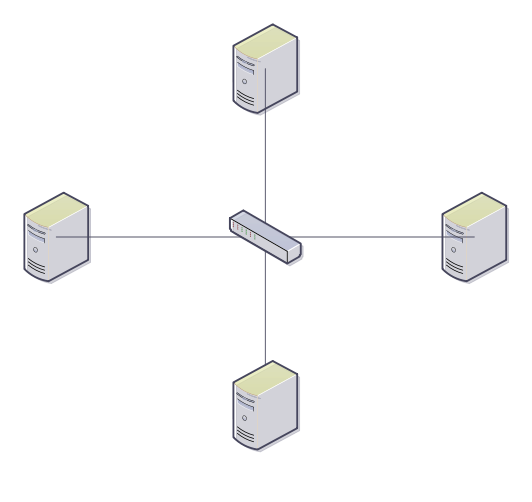
\includegraphics[width=0.6\linewidth]{topologia_gwiazdy}
\caption{Schemat topologii gwiazdy.}
\label{fig:star-network}
\end{figure}

\section{Komunikacja pomiędzy elementami systemu} % (fold)
\label{sec:komunikacja_pomi_dzy_elementami_systemu}
Aplikacja internetowa oraz baza danych umieszczone są na tym samym serwerze. Back-end aplikacji internetowej jest usługą sieciową zrealizowaną w stylu architektury oprogramowania typu REST, która udostępnia interfejsy komunikacyjne dla warstwy prezentacji aplikacji webowej oraz innych aplikacji, np. aplikacji mobilnej na platformę Android, przy pomocy formatu JSON.

Przykładowe zapytanie zwracające podstawowe dane na temat systemu ma następujący przebieg:
\begin{enumerate}
	\item klient webowy wykonuje zapytanie HTTP GET na adres /dashboard.json,
	\item serwer odbiera zapytanie i na tej podstawie wywołuje funkcję odpowiedzialną za pobranie z bazy danych oraz przetworzenie tych danych, 
	\item rezultat wywołanej funkcji zapisywany jest w formacie JSON i odesłany jako odpowiedź.
\end{enumerate}

Główną zaletą podejścia RESTowego jest ogromna skalowalność aplikacji oraz, w pewnym sensie, jej niezależność. Skalowalność aplikacji polega na tym, że system może być w łatwy sposób rozbudowany, niezależność zaś oznacza, że dla klienta serwer jest czarną skrzynką, do której jest podłączony. W trakcie jego działania możliwa jest zmiana algorytmu przetwarzania danych, bądź też całego back-endu, a mimo wszystko dopóki dane wejściowe i wyjściowe będą takie same – nie odczuje on różnicy. Dodatkowo, gdy wystawiona jest jedna wersja API, można równolegle pracować nad drugą, przykładowo: API v1 wystawione jest dla użytkowników aplikacji klienckiej w wersji $<2.0$, natomiast API v2 obsługuje aplikacje w wersji $\ge2.0$. Dzięki temu możliwy jest rozwój aplikacji z jednoczesnym wsparciem wersji poprzednich. 
% section komunikacja_pomi_dzy_elementami_systemu (end)

\chapter{Specyfikacja systemu}
\section{API serwera}
Serwer powinien być rozumiany jako główny element logiki biznesowej systemu. Jest on elementem, który z zewnątrz jest czarną skrzynką, z której korzystają klienci aplikacji androidowej i webowej. Komunikuje się on z innymi systemami w sposób opisany w punkcie \ref{sec:komunikacja_pomi_dzy_elementami_systemu}.

Poza komunikacją z systemami zewnętrznymi, serwer komunikuje się przede wszystkim bezpośrednio z bazą danych. Jest on miejscem, w którym przeprowadzane są wszystkie operacje pobierania, modyfikowania oraz zapisywania danych do bazy.

\section{Aplikacja internetowa}
W tym punkcie jako aplikacje internetową należy rozumieć część aplikacji webowej nazywaną ,,front-end’em'', czyli części służącej do komunikacji z użytkownikiem,przez przeglądarkę internetową.

Aplikacja webowa została napisana za pomocą framework’a AngularJS. Angular ułatwia podział aplikacji zgodnie ze schematem Model-View-Contoller.

Po zalogowaniu do aplikacji wykorzystujemy maszyne stanów adresów, dzięki czemu możliwe jest ładowanie tylko części strony pod paskiem nawigacyjnym, a pasek nawigacyjny zawiera przyciski ładujące odpowiedni widok.

Angular wykorzystuje serwisy do wysłania zapytań do API serwera. Serwisy są asynchroniczne i wykonują się w osobnym wątku. Dzięki takiemu rozwiązaniu użytkownik ma wrażenie ze strona ładuje się natychmiastowo, ponieważ widać jej część, a tak naprawdę większość komponentów czeka na dane zwrócone z API serwera.

Aplikacja internetowa jest w pełni przetłumaczona na język polski oraz angielski. Strona wyświetla się w danym języku na podstawie ustawień przeglądarki.

\chapter{Wybrane technologie}
\section{Hardware}
\section{Software}
\subsection{Aplikacja internetowa}
Serwis internetowy wykonany został w oparciu o następujące technologie:
\begin{itemize}
	\item \textbf{Ruby on Rails} - wnętrze (back-end) portalu webowego, które odpowiedzialne jest za wykonywanie określonych zadań na podstawie danych otrzymanych z fasady (front-end),
	\item \textbf{AngularJS} - fasada (front-end) - jej zadaniem jest komunikacja z użytkownikiem (odbieranie od niego danych oraz przekazywanie ich do back-end'u). AngularJS jest frameworkiem JavaScript'owym, który wymaga stosowania wzorca projektowego \emph{MVC} (ang. Model-View-Controller).
\end{itemize}
Ponadto wykorzystane zostały następujące elementy:
\begin{itemize}
	\item \textbf{CoffeeScript} - język programowania kompilowany do JavaScriptu. Ponieważ CoffeeScript kompiluje się do JavaScriptu, programy mogą być krótsze o około $\frac{1}{3}$ bez strat dla szybkości działania,
	\item \textbf{Slim} – język oparty na szablonach (ang. template language), którego celem jest maksymalna redukcja składni HTML’owej poprzez usunięcie np. tagów zamykających. W efekcie otrzymujemy bardzo czytelny kod, oparty na wcięciach.
\end{itemize}

\subsection{Aplikacja serwerowa} % (fold)
\label{sub:aplikacja_serwerowa}

% subsection aplikacja_serwerowa (end)

\subsection{Baza danych}
Jako system bazodanowy wykorzystany został MySQL w wersji 5.6. Niewątpliwymi zaletami tego systemu jest to, że posiada on wysoki stopień niezawodności, jest darmowy oraz powszechnie dostępny i wspierany.

\chapter{Implementacja}
\chapter{Testy}
\section{Aplikacja internetowa}
\subsection{Testy jednostkowe}
Do testów jednostkowych dla aplikacji webowej użyliśmy biblioteki RSpec, służącej do testowania kodu Rubiego, ze wsparciem dla frameworka Rails. Wybraliśmy tą bibliotekę, ponieważ wspiera ona idee Model-View-Controller, w oparciu o którą powstała nasza aplikacja. Dużą wygodą jest również automatyczna konfiguracja środowiska testowego, która polega m. in.  na osobnej, testowej bazie danych, która jest tworzona na początku wykonywania testów i czyszczona po zakończeniu każdego przypadku testowege.

RSpec posiada bardzo intuicyjną składnie, przyjazna użytkownikowi naszym zdaniem. Testy podzielone są na 3 poziomową strukturę, każdy poziom zaczyna się słowem kluczowym:
\begin{enumerate}
	\item ,,describe'' – tu definiujemy jaką funkcje/klasę/moduł ma sprawdzać dany zbiór testów,
	\item ,,context'' – to miejsce służy do określenia warunków testu,
	\item ,,it'' – mówi nam jak powinien się zachować testowany moduł.
\end{enumerate}

Przykładowy pojedynczy przypadek testowy:

\begin{lstlisting}[language=Ruby, caption={RSpec test jednostkowy.}]
RSpec.describe TripsController, :controller do #
Describe'POST #create' do
context 'with valid attributes' do
it 'creates the trip' do
login_user
post :create, trip: attributes_for(:trip_with_path), format: :json
expect(Trip.count).to eq(1)
end
end
end
end
\end{lstlisting}

Powyższy test ma za zadanie sprawdzić czy dane wysłane w odpowiednim formacie zapytaniem http post, przekazane do funkcji ,,create'' klasy ,,TripsController'' stworzą w bazie danych nowy rekord w tabeli Trip. 

Dla ułatwienia wprowadzania atrybutów do testowanych metod lub dodawania rekordów do bazy danych nie wykorzystując napisanych przez siebie metod posłużyliśmy się biblioteką ,,FactoryGirl'', która implementuje wzorzec projektowy fabryki. Definicja obiektu jest bardzo prosta:

\begin{lstlisting}[language=Ruby, caption={Definicja FactoryGirl.}]
FactoryGirl.define do 
factory :full_trip, class: Trip do
distance 100
avg_rpm 2500
avg_speed 94
avg_fuel 8.9
date '2015-05-14T21:23:11.510Z'
mark 5.0
user_id 1
beginning 'Start'
finish 'Finish'
challenge_id nil
engine_type_id 1
engine_displacement_id 1
end
end
\end{lstlisting}

Poniżej znajduje się użycie metody "FactoryGirl.create'', która tworzy obiekt w bazie danych. Ten przykład ilustruje również strukturę zbioru testów dla pojedynczej metody:

\begin{lstlisting}[language=Ruby, caption={Użycie FactoryGirl.}]
describe 'GET #mytrips' do
context 'with valid attributes' do
let!(:login) { login_user }
let(:current_user_id) { login.id }
it 'renders all user\'s trips as json' do
FactoryGirl.create(:engine_displacement)
FactoryGirl.create(:engine_type)
FactoryGirl.create(:fuel_consumption)
FactoryGirl.create(:full_trip, user_id: current_user_id)
get :mytrips, format: :json
expect(response).to be_success
json = JSON.parse(response.body)
expect(json).not_to be_empty
expect(json[0].length).to eq(20)
end
it 'renders empty array when user has no trips' do
get :mytrips, format: :json
expect(response).to be_success
json = JSON.parse(response.body)
expect(json).to be_empty
end
end

context 'with user not logged in' do
it 'redirects to login page' do
FactoryGirl.create(:engine_displacement)
FactoryGirl.create(:engine_type)
FactoryGirl.create(:full_trip)
get :mytrips, format: :json
expect(response).to have_http_status(401)
end
end
end
\end{lstlisting}

Stworzyliśmy 19 testów jednostkowych. Badaliśmy pokrycie kodu aplikacji testami narzędziem Rcov. Tą analizę uruchamialiśmy po każdym commicie do repozytorium, dlatego wiemy jak się to kształtowało od moment skonfigurowania Rcov w Jenkinsie:
\begin{figure}[h]
	\centering
	%\includegraphics[width=0.8\linewidth]{}
	\caption{Wykres pokrycia kodu.}
	\label{fig:testy}
\end{figure}

Ostatecznie pokrycie kodu źródłowego testami jednostkowymi wynosi około 75\%. Rcov pokazuje również dokładnie, które linie kodu są testowane:
\begin{figure}[h]
	\centering
	%\includegraphics[width=0.9\linewidth]{}
	\caption{Raport Rcov dla pliku trips\_controller.rb.}
	\label{fig:raport}
\end{figure}
\chapter{Podsumowanie}

\begin{thebibliography}{inteligencja}
	\addcontentsline{toc}{chapter}{Bibliografia}
	
	\bibitem{rails guide}
	\emph{Ruby on Rails Guides}, dostępne pod adresem: \url{http://guides.rubyonrails.org/},\\ aktualne na dzień 14.06.2015r.
	
	\bibitem{angular guide}
	\emph{AngularJS Developer Guide}, dostępne pod adresem: \url{https://docs.angularjs.org/guide}, aktualne na dzień 14.06.2015r.

	\bibitem{inteligentne domy}
	Piątek Z., \emph{Od automatyki budynkowej do inteligentnych domów}, dostępne pod adresem \url{http://automatykab2b.pl/}, aktualne na dzień 31.10.2015r.

	\bibitem{magisterka}
	Płachta K., \emph{System komunikacyjny w inteligentnym budynku}, 2012

	\bibitem{cleancode}
	Martin, R. \emph{Czysty kod. Podręcznik dobrego programisty}, Gliwice, Wydawnictwo Helion 2010
	
\end{thebibliography}
\end{document}